\section{Introduction}
The algorithms presented in this paper were implemented in \texttt{C++} using NetworKit and Koala libraries. The source code is submitted as a part of the Koala-NetworKit GitHub repository: \url{https://github.com/krzysztof-turowski/koala-networkit/pull/45}.

The algorithms and the soft heap are implemented in these files:
\begin{itemize}
    \item \texttt{include/mst/MinimumSpanningTree.hpp}
    \item \texttt{cpp/mst/MinimumSpanningTree.cpp}
    \item \texttt{include/structures/heap/SoftHeap.hpp}
\end{itemize}


\section{Results}
\subsection{Dataset}
Three primary datasets were used for testing purposes were road maps of the New York city, the Great Lakes Area and Florida respectively, where the edge weights represent distances. 

For the purpose of testing the randomized Chazelle-Rubinfeld-Trevisan algorithm five new graphs each were created from them with edge weights preprocessed so that $w_e' = \max\{w, \left\lceil \frac{w_e}{200}\right\rceil\} \text{ for } w \in \{15, 31, 63, 127, 255\}$. The runtime of that algorithm is dependent on the maximum edge weight in the graph and these datasets have large edge values.

For the purpose of testing Chazelle's determinisitc algorithm the three graphs were preprocessed so that they are connected and the all edges have distinct costs.

\subsection{Chazelle's algorithm}
\begin{table}[ht!]
  \centering
  \begin{tabular}{|c|c|c|c|c|c|}
    \hline
    Graph $G$ & $|V(G)|$ & $|E(G)|$ & \textsc{Chazelle} & \textsc{Bor\r{u}vka} & Time difference \\ \hline
    New York & 264346 & 733846  & 957 & 646 & 48\% \\ \hline
    Florida & 1070376 & 2712798  & 4157 & 3126 & 33\%  \\ \hline
    Lakes & 2758119 & 6885658 & 13803 & 10292 & 34\% \\ \hline
    \end{tabular}
  \caption{Comparison of Chazelle's and Bor\r{u}vka's algorithms. Time in ms.}
  \label{t1}
\end{table}
\FloatBarrier

As we can see from the \Cref{t1} my implementation of the Chazelle's algorithm is slower then the Bor\r{u}vka's algorithm. It is to be expected as Chazelle's algorithm uses the Bor\r{u}vka's algorithm as a subroutine and in the time it takes to construct the $T$ hierarchy several \textsc{Boruvka-step}s could be performed. Notice that the graphs are small enough so that the number of \textsc{Boruvka-step}s necessary to compute the minimum spanning tree is at most $22$. 

\subsection{Chazelle-Rubinfeld-Trevisan algorithm}

On each of the $3$ datasets the algorithm was run with all possible pairs of values $\epsilon \in \{0.1, 0.05, 0.03, 0.02, .01\}$ and $x \in \{15, 31, 63,  127, 255\}$. Each configuration was run 5 times and the time and MST weight values used to create tables and plots were averaged over these 5 runs. 

I will first show the tables and plots and analyze them at the end.

\begin{table}[ht!]
  \centering
  \begin{tabular}{|c|c|c|c|c|c|c|}
    \hline
    $x \backslash \epsilon$ & 0.1 & 0.05 & 0.03 & 0.02 & 0.01 & \textsc{Bor\r{u}vka} \\ \hline
    \multicolumn{7}{|c|}{\textbf{New York City}} \\ \hline
    15 & 2.1 & 7.6 & 19.2 & 45.0 & 175.0 & 1129.0 \\ \hline
    31 & 5.8 & 17.7 & 51.7 & 115.2 & 492.2 & 1125.4 \\ \hline
    63 & 10.9 & 40.7 & 112.2 & 269.7 & 1175.8 & 1121.4 \\ \hline
    127 & 21.7 & 80.2 & 239.6 & 565.3 & 2503.0 & 1100.3 \\ \hline
    255 & 46.1 & 175.4 & 525.9 & 1257.3 & 5323.3 & 1136.4 \\ \hline
    \multicolumn{7}{|c|}{\textbf{Florida}} \\ \hline
    15 & 2.2 & 7.1 & 17.6 & 38.0 & 151.6 & 4579.7 \\ \hline
    31 & 5.3 & 18.2 & 49.2 & 109.5 & 470.7 & 4528.7 \\ \hline
    63 & 12.2 & 43.9 & 124.2 & 280.1 & 1241.8 & 4731.2 \\ \hline
    127 & 23.9 & 92.3 & 268.5 & 631.7 & 2807.5 & 4722.7 \\ \hline
    255 & 49.8 & 195.1 & 578.4 & 1383.7 & 5964.4 & 4708.8 \\ \hline
    \multicolumn{7}{|c|}{\textbf{Great Lake Area}} \\ \hline
    15 & 3.1 & 8.2 & 20.0 & 41.0 & 156.7 & 12620.3 \\ \hline
    31 & 6.7 & 21.8 & 63.0 & 129.7 & 631.7 & 13855.9 \\ \hline
    63 & 14.5 & 52.5 & 155.2 & 382.2 & 1449.4 & 14445.3 \\ \hline
    127 & 30.5 & 112.9 & 333.3 & 768.9 & 3303.6 & 14053.5 \\ \hline
    255 & 60.4 & 246.2 & 704.1 & 1663.2 & 7228.6 & 13955.5 \\ \hline
  \end{tabular}
  \caption{Average time in ms.}
\end{table}

\begin{table}[ht!]
  \centering
  \begin{tabular}{|c|c|c|c|c|c|}
    \hline
    $x \backslash \epsilon$ & 0.1 & 0.05 & 0.03 & 0.02 & 0.01 \\ \hline
    \multicolumn{6}{|c|}{\textbf{New York City}} \\ \hline
    15 & 0.0144 & 0.0071 & 0.0055 & 0.0048 & 0.0021 \\ \hline
    31 & 0.0090 & 0.0063 & 0.0027 & 0.0046 & 0.0019 \\ \hline
    63 & 0.0141 & 0.0084 & 0.0028 & 0.0037 & 0.0010 \\ \hline
    127 & 0.0148 & 0.0058 & 0.0065 & 0.0049 & 0.0015 \\ \hline
    255 & 0.0142 & 0.0073 & 0.0039 & 0.0024 & 0.0021 \\ \hline
    \multicolumn{6}{|c|}{\textbf{Florida}} \\ \hline
    15 & 0.0224 & 0.0121 & 0.0068 & 0.0036 & 0.0021 \\ \hline
    31 & 0.0095 & 0.0107 & 0.0077 & 0.0027 & 0.0014 \\ \hline
    63 & 0.0222 & 0.0096 & 0.0017 & 0.0020 & 0.0017 \\ \hline
    127 & 0.0166 & 0.0084 & 0.0032 & 0.0031 & 0.0013 \\ \hline
    255 & 0.0169 & 0.0119 & 0.0089 & 0.0051 & 0.0014 \\ \hline
    \multicolumn{6}{|c|}{\textbf{Great Lake Area}} \\ \hline
    15 & 0.0108 & 0.0067 & 0.0035 & 0.0021 & 0.0013 \\ \hline
    31 & 0.0173 & 0.0070 & 0.0101 & 0.0039 & 0.0016 \\ \hline
    63 & 0.0198 & 0.0160 & 0.0012 & 0.0033 & 0.0014 \\ \hline
    127 & 0.0124 & 0.0043 & 0.0049 & 0.0016 & 0.0027 \\ \hline
    255 & 0.0216 & 0.0043 & 0.0029 & 0.0027 & 0.0013 \\ \hline
  \end{tabular}
  \caption{Average absolute relative error}
\end{table}

\begin{figure}[H]
    \centering
    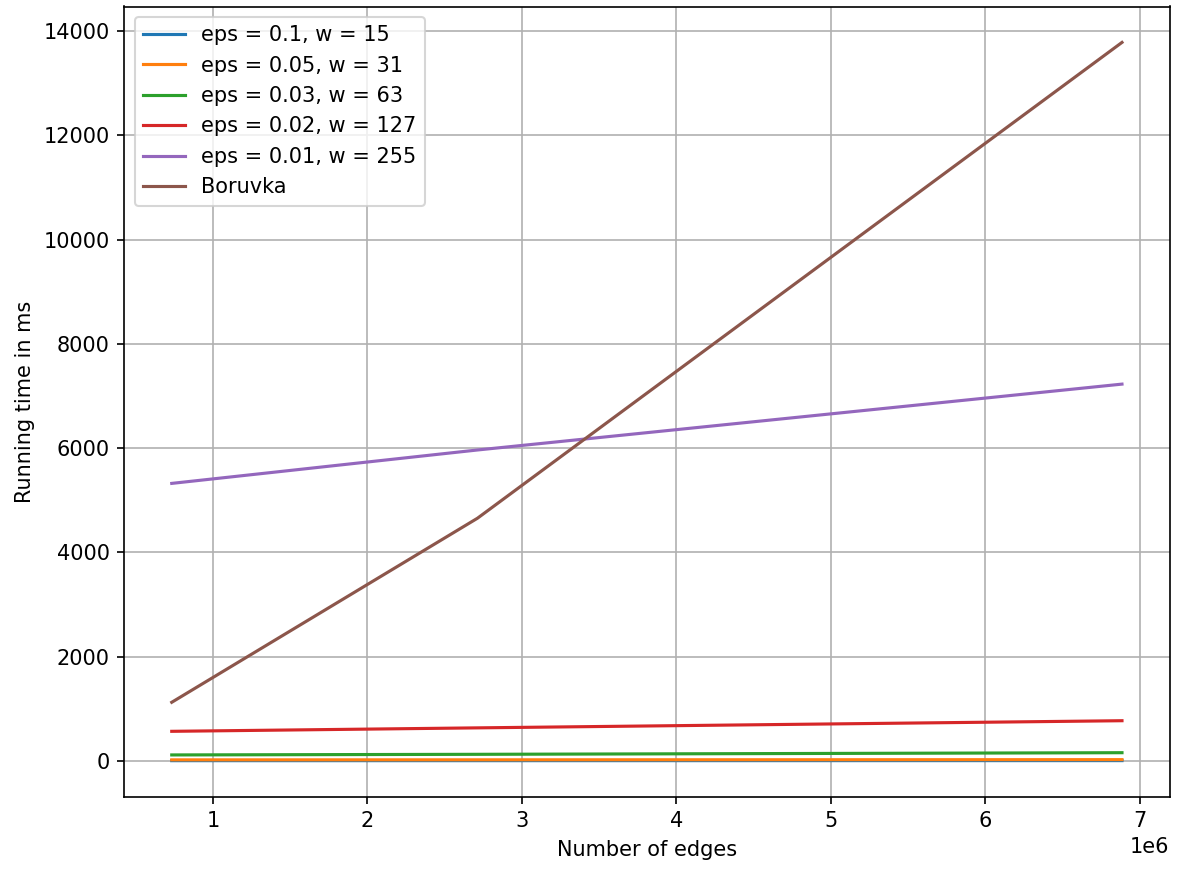
\includegraphics[width=1\linewidth]{figures/DifferentInputGraphs.png}
    \caption{Comparison of the CRT and Bor\r{u}vka algorithms across all datasets.}
    \label{fig:cmp}
\end{figure}
\FloatBarrier

\begin{figure}[H]
    \centering
    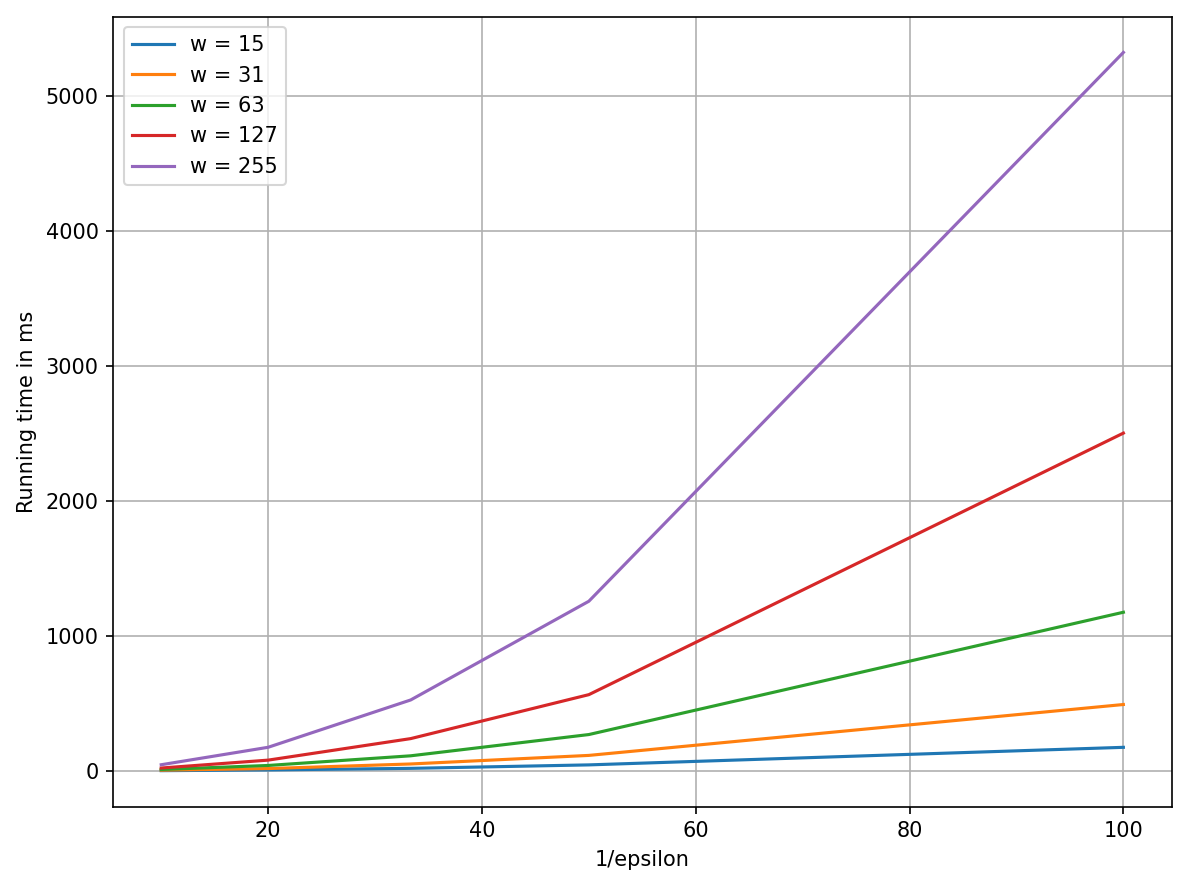
\includegraphics[width=0.9\linewidth]{figures/NYDifferentEpsilons.png}
    \caption{Comparison of the CRT algorithm run on the New York City road map graph processed with different $w$ values.}
    \label{fig:nyeps}
\end{figure}
\FloatBarrier

\begin{figure}[H]
    \centering
    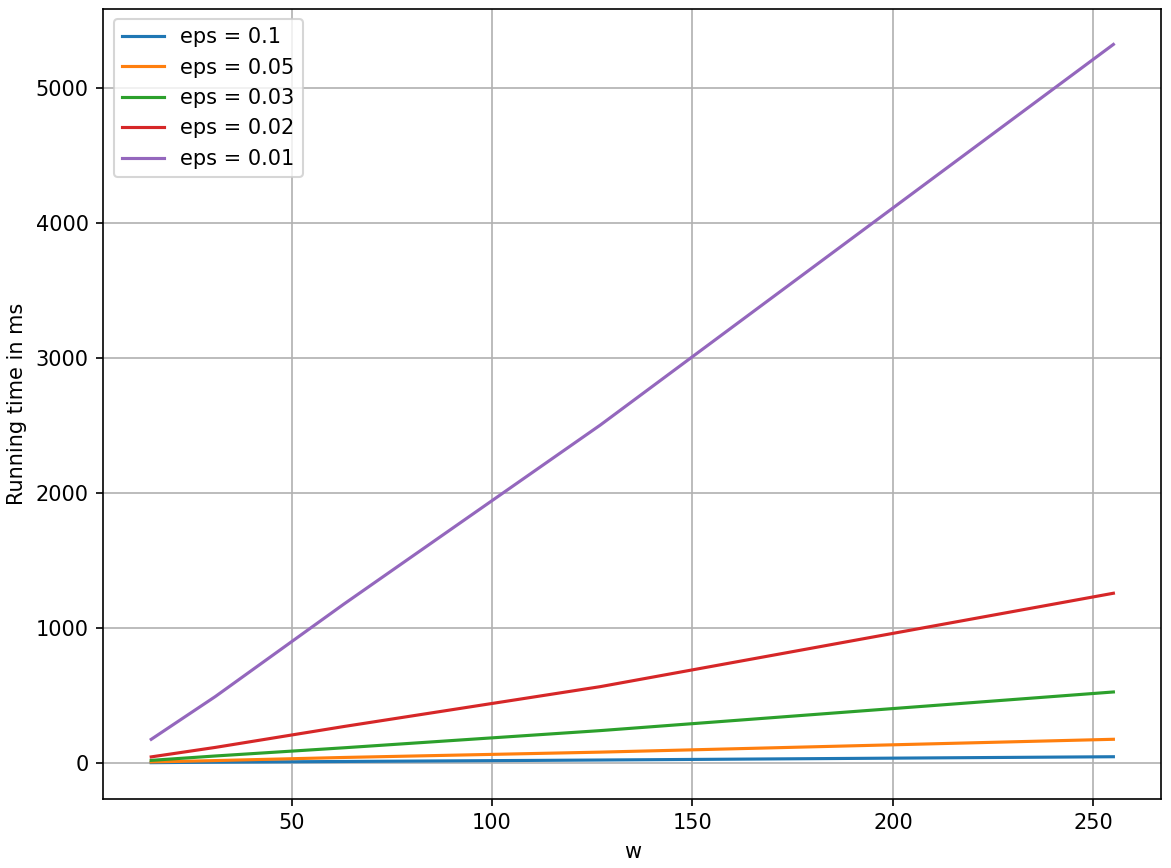
\includegraphics[width=0.9\linewidth]{figures/FLADrifferentWs.png}
    \caption{Comparison of the CRT algorithm run with different $\epsilon$ values on the Florida road map graph processed with different $w$ values.}
    \label{fig:flaws}
\end{figure}

Looking at the results it is evident that Chazelle-Rubinfeld-Trevisan algorithm clearly outperform Borůvka's on most of the test cases. Focusing on the New York City graph we can see that the randomized algorithm provided accurate (relative error is much smaller then $\epsilon$) results and finished much faster then the deterministic one, but for the most computationally intensive cases with $(\epsilon, w) \in \{(0.01, 255), (0.01, 127), (0.01, 63), (0.02, 255)\}$.

Remember that the expected time complexity of the Chazelle-Rubinfeld-Trevisan algorithm is $O(dw\epsilon^{-2}\log \frac{dw}{\epsilon})$. We will consider what happens when we fix the $\epsilon$ or the $w$ parameter. 

Fixing the $\epsilon$ value for a given graph shows that the algorithm running times grow slightly faster than a linear function in terms of $w$, that is, the maximum edge cost. This is illustrated by the columns of the average times tables or \Cref{fig:nyeps}.

On the other hand fixing the $w$ for a given graph clearly shows a superlinear growth when plotted against the $\epsilon^{-1}$ that might indeed be $O(\epsilon^{-2}\log{\epsilon^{-1}})$ -- as \Cref{fig:flaws} shows.

\Cref{fig:cmp} shows how the Chazelle-Rubinfeld-Trevisan runtime is affected by increasing the graph size. It is important to note that the average degrees in the input graphs are $5.55, 5.07, 4.99$ respectively, so while the number of edges rises, the average degree falls however slightly. Based on the complexity alone we should expect the running time to be slightly better for the bigger graphs. One possible explanation for the runtime growing slowly could be the hardware. Larger graph means that more calls to the memory result in cache misses as lower fraction of the data will fit in the caches.

\section{Finishing thoughts}

Chazelle's deterministic algorithm turned out to be more complex and slower in practice then Borůvka's algorithm. This was expected, since despite its superior theoretical complexity, the algorithm relies on multiple costly passes and recursive steps that make it less practical.

Chazelle, Rubinfeld and Trevisan algorithm displays promising results for computing the MST weight of graphs with small edge costs and with low precision. It outperformed Borůvka's algorithm significantly in most of the test cases. Modifying the graph by scaling the edge costs down or capping them at some maximum value can be useful to reduce the running time of the approximate algorithm, but it may change the MST weight drastically, far more then in the $\epsilon$ relative error range.
